\documentclass[border=10pt]{standalone}

\usepackage{tikz}
\usepackage{tikzsymbols}
\usetikzlibrary{calc,patterns,shapes.geometric}

\def\centerarc[#1](#2)(#3:#4:#5){\draw[#1] ($(#2)+({#5*cos(#3)},{#5*sin(#3)})$) arc (#3:#4:#5);}

\begin{document}
	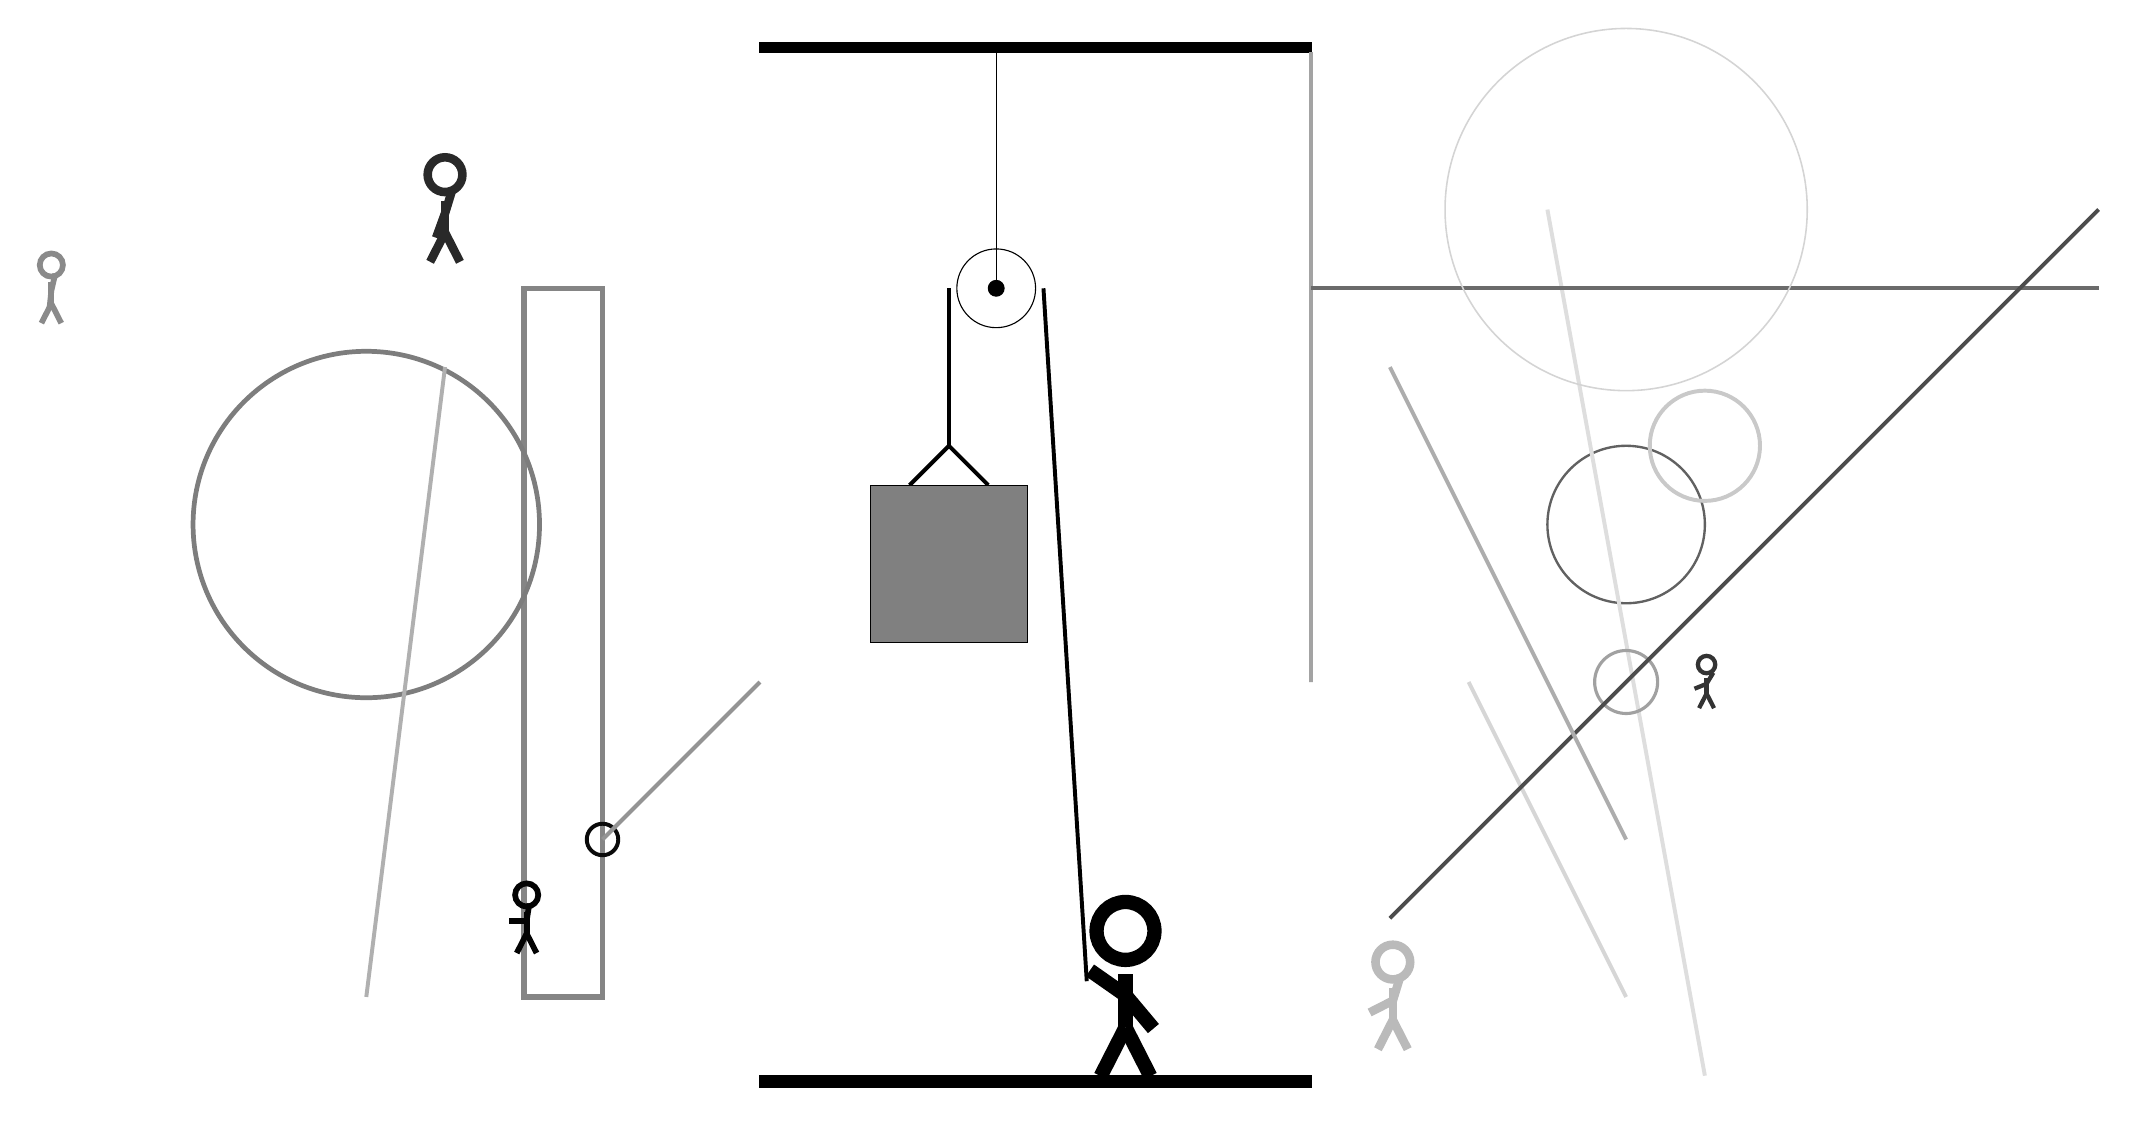
\begin{tikzpicture}
		%%%%% START %%%%%
		
		\draw[fill=black] (-2, 10) rectangle (5, 10.125);
		
		\draw (1, 7) circle (0.5);
		\draw[fill=black] (1, 7) circle (0.1);
		\draw (1, 10) -- (1, 7);
		
		\draw[line width=0.5mm] (-0.1, 4.5) -- (0.4, 5.0) -- (0.9, 4.5);
		\draw[fill=black!50] (-0.6, 4.5) rectangle (1.4, 2.5);
		
		\draw[line width=0.5mm] (0.4, 7) -- (0.4, 5.0);
		\centerarc[line width=0.5mm](1, 7)(0:180:0.6);
		\draw[line width=0.5mm](1.6, 7) -- (2.15, -1.8);
		
		\draw[line width=0.5mm, color=black!36] (5, 10) rectangle (5, 2);
		
		\draw [line width=0.3mm, color=black!62](9, 4) circle (1.0);
		\draw[line width=0.5mm, color=black!16](9, -2) -- (7, 2);
		\draw[line width=0.7mm, color=black!48] (-4, -2) rectangle (-5, 7);
		\draw[line width=0.5mm, color=black!13](8, 8) -- (10, -3);
		
		\draw [line width=0.5mm, color=black!21](10, 5) circle (0.7);
		
		\node[line width=0.4mm, color=black!46] at (-11, 7) {\Strichmaxerl[4][84][77]};
		\draw [line width=0.4mm, color=black!37](9, 2) circle (0.4);
		\draw [line width=0.5mm, color=black!96](-4, 0) circle (0.2);
		\draw [line width=0.6mm, color=black!51](-7, 4) circle (2.2);
		\draw[line width=0.5mm, color=black!58](5, 7) -- (15, 7);
		\node[line width=0.4mm, color=black!84] at (-6, 8) {\Strichmaxerl[6][70][73]};
		\node[line width=0.3mm, color=black!80] at (10, 2) {\Strichmaxerl[3][22][59]};
		
		\draw[line width=0.5mm, color=black!70](6, -1) -- (15, 8);
		\draw[line width=0.5mm, color=black!42](-4, 0) -- (-2, 2);
		\node[line width=0.5mm, color=black!99] at (-5, -1) {\Strichmaxerl[4][0][81]};
		
		\draw[line width=0.5mm, color=black!32](6, 6) -- (9, 0);
		\draw[line width=0.5mm, color=black!31](-6, 6) -- (-7, -2);
		\node[line width=0.5mm, color=black!27] at (6, -2) {\Strichmaxerl[6][27][73]};
		\draw [line width=0.2mm, color=black!17](9, 8) circle (2.3);
		
		\node at (2.6, -1.9) {\Strichmaxerl[10][-35][-50]};
		
		\draw[fill=black] (-2, -3) rectangle (5, -3.15);
		
		%%%%% END %%%%%
	\end{tikzpicture}
\end{document}